\documentclass[letterpaper,12pt]{article}

\usepackage{graphicx}
\graphicspath{{./images/}}
\usepackage{amssymb}
\usepackage{amsmath}
\usepackage{amstext}
\usepackage{subfigure}
\usepackage{url}
\usepackage{color}
\usepackage{hyperref} \hypersetup{pdfborder={0 0 0}}
\usepackage{circuitikz}
\usepackage[framemethod=tikz]{mdframed}
\usepackage{anyfontsize}

\newcommand{\argmax}[1]{\operatorname*{argmax}_{#1}}
%%%
\newmdenv[
linewidth=1pt,
innerrightmargin=80pt,
singleextra={
  \path let \p1=(P), \p2=(O) in
  node[xshift=-40pt] at (P|-0,0.5*\y1+0.5*\y2)
    {\fontsize{100}{120}\selectfont ?};
}
]{Qbox}

\newcommand\questionbox[1]{%
  \begin{Qbox}#1\end{Qbox}}
%%%


\addtolength{\oddsidemargin}{-.875in}
\addtolength{\evensidemargin}{-.875in}
\addtolength{\textwidth}{1.75in} \addtolength{\topmargin}{-.875in}
\addtolength{\textheight}{1.75in} \special{papersize=\the\paperwidth,\the\paperheight}

\begin{document}

\begin{table}[h]
\begin{tabular}{cc}
  
\includegraphics[width=2in,keepaspectratio=true]{images/logo.eps} &
  \begin{tabular}{c}
    \vspace*{0.5cm}{\large ECE4305: Software-Defined Radio Systems and Analysis} \\
    \vspace*{0.1cm}{\large Laboratory 3: Frame Synchronization} \\
  \end{tabular}\\
  \hline
\end{tabular}
\end{table}

\section*{Objective} This laboratory will introduce the concept of frame synchronization between transmitting 
and receiving nodes. Specifically, a simplified error model will be discussed along with an efficient
method with various implementations. Moreover, MATLAB\textregistered~will also be introduced as development 
tools for digital communication systems, especially the construction of a prototype software-defined radio 
(SDR) based simulation.
\tableofcontents

\newpage

\section{Theoretical Preparation}
The fundamental concepts of digital communication systems and related theoretical background material covered in this section will serve as a basis for the implementation and design of prototype systems throughout the rest of this course.

\subsection{O Frame, Where Art Thou?}\label{sec:models}
%
In previous labs we have discussed frequency correction, timing compensation, and matched filtering.  The 
final aspect of synchronization is frame synchronization.  At this point it is assumed that the available 
samples represent single symbols and are corrected for timing, frequency, and phase offsets. However, since 
in a realistic system the start of a frame will still be unknown, we  need to perform an additional 
correction. We demonstrate this issue visually in Figure~\ref{fig:frame_offset2}, which contains a sample 
synchronized frame with an unknown offset of $p$ samples.
%
\begin{figure}[ht!]\label{fig:frame_offset2}
 \centering
 \includegraphics[width=0.8\textwidth]{frameOffset.eps}
\caption{Example received frame in AWGN with an unknown sample offset.}
\end{figure} 
%
Once we have an estimate $\hat{p}$ we can extract data from the desired frame, demodulated to bits, and 
perform any additional channel decoding or source decode originally applied to the signal.  There are various way to accomplish this estimation but the implemented outlined in this lab is based around cross-correlation.\par

%\newpage
\section{Frame Synchronization}\label{sec:timing}
%
The common method of determining the start of a given frame is with the use of markers, even in wired 
networking.  However, in the case of wireless signals, this problems becomes more difficult as made visible 
in Figure~\ref{fig:frame_offset2} which actually uses a marker.  Due to the high degree of noise content in 
the signal, specifically designed preamble sequences are appended to frames before modulation.  Such 
sequences are typically known exactly at the receiver and have certain qualities that make frame estimation 
accurate.  In Figure~\ref{fig:frame_structure} we outline a typical frame ordering containing: preamble, 
header, and payload data.  Header and payloads are unknown are the receiver, but will maintain some structure 
so they can be decoded correctly.\par
%
\begin{figure}[ht!]\label{fig:frame_structure}
 \centering
 \includegraphics[width=0.8\textwidth]{Preamble-crop.pdf}
\caption{Common frame structure of wireless packet with preamble followed by header and payload data.}
\end{figure} 
%
Before we discuss the typical sequences utilized we will introduce a technique for estimation of the start of 
a known sequence starting at an unknown sample in time. Let us consider a set of $N$ different 
binary sequences $y_n$, where $n \in \big[1,...,N\big]$, each of length $L$.  Given an additional 
binary sequence $x$, we want to determine how similar $x$ is to the existing $N$ sequences.  The use of a 
cross-correlation would provide us the appropriate estimate, which we perform as:
%
\begin{equation}
  C_{xy}(k) = \sum_{m}x^{*}(m)y_n(m+k),
\end{equation}
%
which is identical to a convolution without a time reversal on the second term.  When $x=y_n$ for a given 
$n$, $C_{xy}$ will be maximized compared with the other $n-1$ sequences, and produce a peak at 
$L^{\mathrm{th}}$ index at least.  We can use this concept to help build our frame start estimator, which we 
have discussed will contain a known sequence called the preamble.\par
%
Common sequences utilized in preambles for narrowband communications are Barker Codes~\cite{barke1953group}. 
 Barker Codes are utilized since they have unique auto-correlation properties that have minimal or ideal 
off-peak correlation.  Specifically, such codes or sequences $a(i)$ have autocorrelation functions defined as:
\begin{equation}
 c(k) = \sum_{i=1}^{N-k} a(i) a(i+k),
\end{equation}
%
such that:
%
\begin{equation}
 \lvert c(v) \rvert \le 1, \quad 1\le v < N.
\end{equation}
However, only nine sequences are known $N\in\big[1, 2, 3, 4, 5, 7, 11, 13\big]$, provided in 
Table~\ref{tbl:barkercode}.  We provide a visualization of these auto-correlations in 
Figure~\ref{fig:barker_codes}, for a select set of lengths.  As the sequence becomes longer the central peak 
becomes more pronounced.  For communication systems we typically append multiple such codes together to 
produce longer sequences for better performance, as well as for other identifications.\par
%
\begin{figure}[ht!]\label{fig:barker_search}
 \centering
 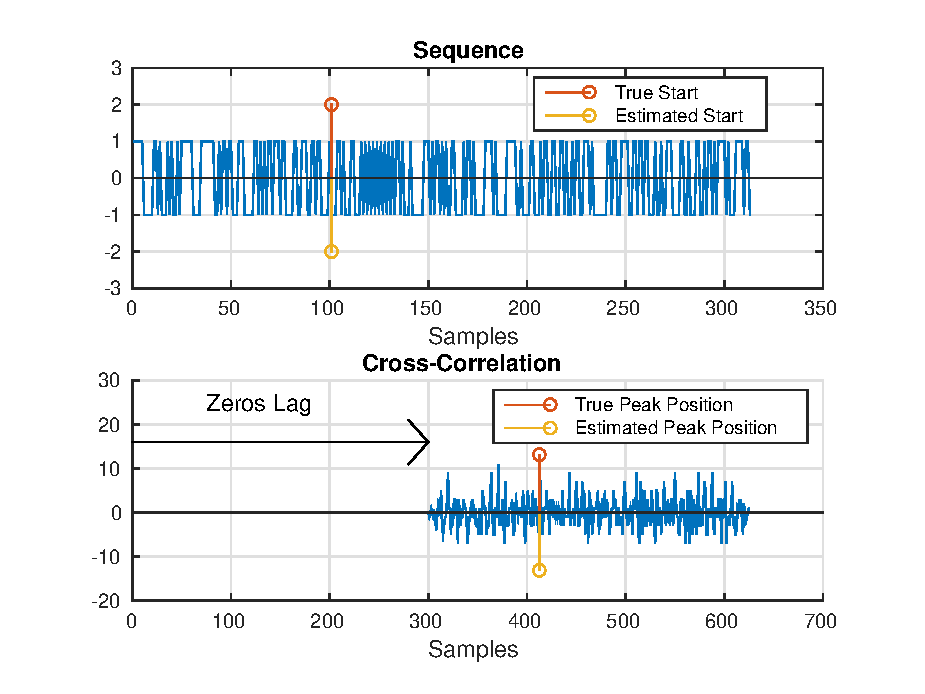
\includegraphics[width=0.8\textwidth]{searchBarker.eps}
\caption{Sample Barker Code implementation for sequence offset determination.}
\end{figure}
%
Using these codes we have implemented a small example to show how a barker sequence $a(k)$ can be used to 
locate sequences in a larger set of data $r(k)$, which we have provided in \texttt{lab3part1.m}.  In this 
example we insert a barker code within a larger random sequence at an unknown position $p$, similar to our 
original error model in Section~\ref{sec:models}, show as the top plot in Figure~\ref{fig:barker_search}.  A 
cross-correlation is performed using MATLAB\textregistered's \texttt{xcorr} function, providing the lower plot 
in Figure~\ref{fig:barker_search}.  The cross-correlation will be of length $2L_r-1$, where $L_r$ is the 
length of $r$. Since \texttt{xcorr} will pad zeros to $a$ so its length is equal to $L_r$~\cite{xcorr}, this 
will result in at least $L_r-L_a$ zeros to appear in the correlation where $L_a$ is the original length of 
$a$.  From Figure~\ref{fig:barker_codes}, we know that the peak will appear at $L_a$ samples from the start 
of the sequence.  Taking this into account we can directly determine at what offset position of our desired 
sequence:
%
\begin{equation}
 \hat{p} = \argmax{k}\,C_{ra}(k) - L_r,
\end{equation}
%
which is what we observe from our estimates in the top plot of Figure~\ref{fig:barker_search}.\par
%
Now that we have a method for estimating the start of a frame, let us consider a slightly simplier problem. 
Can we determine that a frame exist in the correlation?  This can be useful if wish to handle data in smaller 
pieces rather than working with complete frames, or possibly a mechanism for determining if a channel is 
occupied.  When we consider signal detection, we typically define this feature as a power sensitivity, or 
the minimum received power at the receiver to be detected.  However, this sensitivity will be based on some 
source waveform and cannot be generalized.  Therefore, such a value will should never be given on its own, 
unless given with respect to some standard transmission.  Even when considering formal methods of detection 
theory, such as Neyman-Pearson or even Baysian, you must have some knowledge or reference to the source 
signal~\cite{kay1998fundamentals}.  The receiver sensitivity requirement for 802.11ac specifically is defined as 
the minimum received signal power to maintain a packet error rate of $10\%$, for a give modulation and coding 
scheme~\cite{ieee80211ac}.\par
%
When we consider the implementation consequences of detecting a signal, our design become more complicated 
than for example \texttt{lab3part1.m}.  In the most basic sense detection becomes a thresholding problem for 
our correlator.  Therefore, the objective becomes in determining a reference or criteria for validating a 
peak, which can be radically different over time depending on channel noise and the automatic gain control of 
the Pluto.  However, even in simulations appropriate thresholding become non-trivial, which we can 
demonstrate with Figures~\ref{fig:fake} and~\ref{fig:real}.  In these Figures the peak appears larger relative to 
the rest of the correlation in the case where no frame exists in the receive signal, compared to the 
condition when a frame exists.  Therefore, for an implementation that performs well it should handle such 
conditions, and operate no matter the input scaling.\par
%
In \texttt{lab3part2.m} we have enhanced the baseline bit generation to include support for ASCII characters to bits and back to ASCII.  Included as well is an example demodulation and packet error rate measurement.  These will be used to determine overall performance of your receiver design, and frame synchronizer.
%

\begin{figure}
\centering
\begin{minipage}{.5\textwidth}
  \centering
  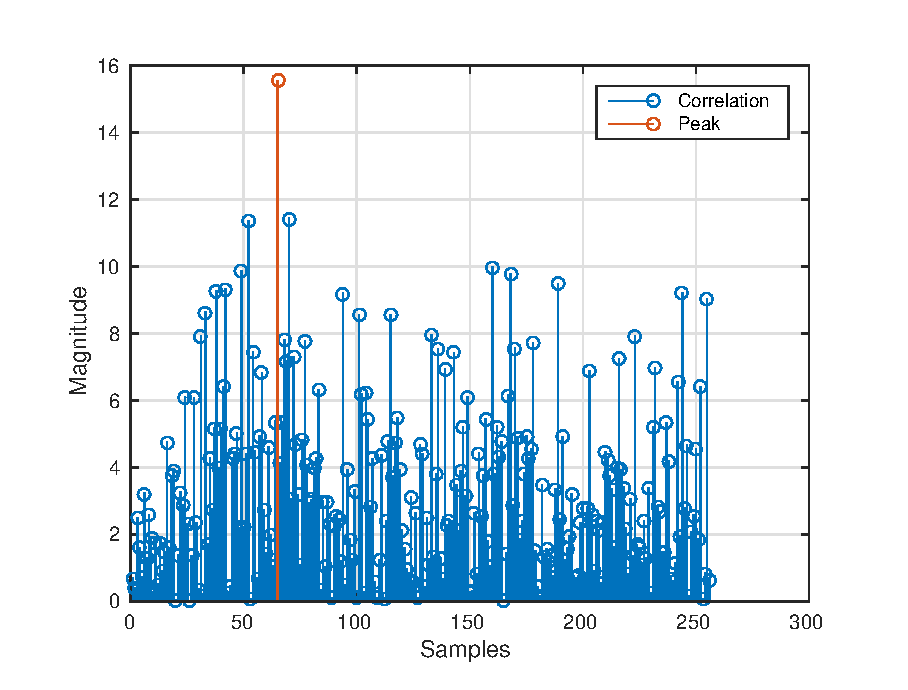
\includegraphics[width=1.0\linewidth]{fake_peak.eps}
  \caption{Correlation without signal present.}
  \label{fig:fake}
\end{minipage}%
\begin{minipage}{.5\textwidth}
  \centering
  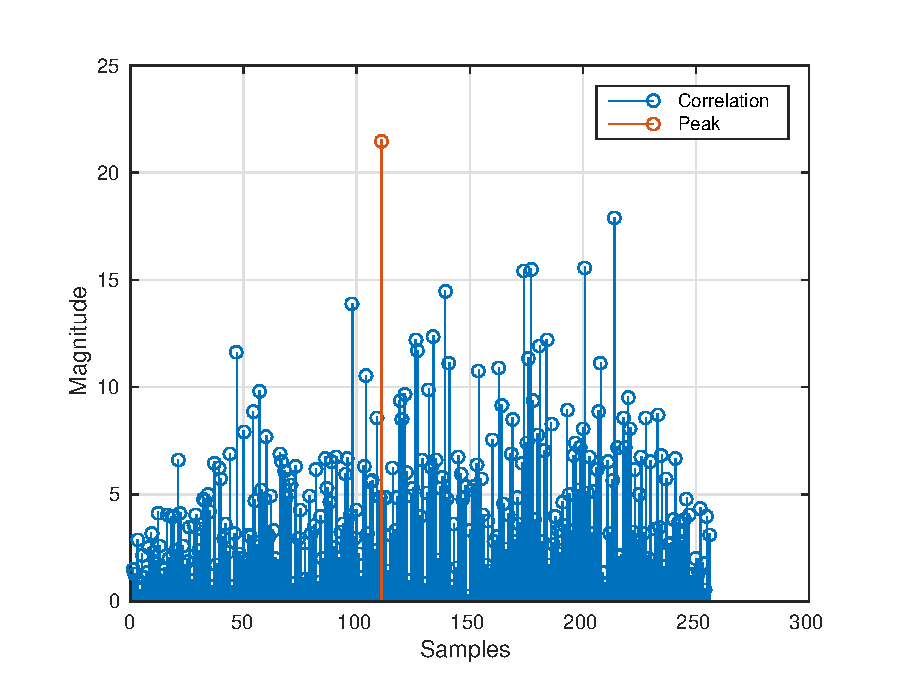
\includegraphics[width=1.0\linewidth]{true_peak.eps}
  \caption{Correlation with signal present.}
  \label{fig:real}
\end{minipage}
\end{figure}

\vbox{
\questionbox{
\begin{itemize}
  \item Question 0: Based on \texttt{lab3part1.m} implement an alternative scheme that utilized the 
\texttt{filter} function for estimation rather than \texttt{xcorr}.  (\texttt{filter} is generally much faster than 
\texttt{xcorr} in interpreted MATLAB.)  Provide a benchmark using \texttt{tic} and \texttt{toc} for their relative performance for different sequence lengths. 
  \item Question 1: Based on template provided in \texttt{lab3part2.m} and the example in \texttt{lab3part1.m} implement a frame synchronization scheme.
  \item Question 2: Test your frame synchronization implementation over the SNR range $\big[0,10\big]$ dB and provide the resulting plot for detection probability and packet error rate.
  \item Question 3: For a coherent modulation scheme (such as QPSK) what modification would be require to 
correctly decode or demodulate the received symbols after the frame has been recovered?  Describe provide two techniques for solving this problem.
\end{itemize}
}
}


\newpage
  %       1           [-1]
  %       2           [-1 1]
  %       3           [-1 -1 1]
  %       4           [-1 -1 1 -1]
  %       5           [-1 -1 -1 1 -1]
  %       7           [-1 -1 -1 1 1 -1 1]
  %       11          [-1 -1 -1 1 1 1 -1 1 1 -1 1]
  %       13          [-1 -1 -1 -1 -1 1 1 -1 -1 1 -1 1 -1]
%
\begin{figure}[ht!]\label{fig:barker_codes}
 \centering
 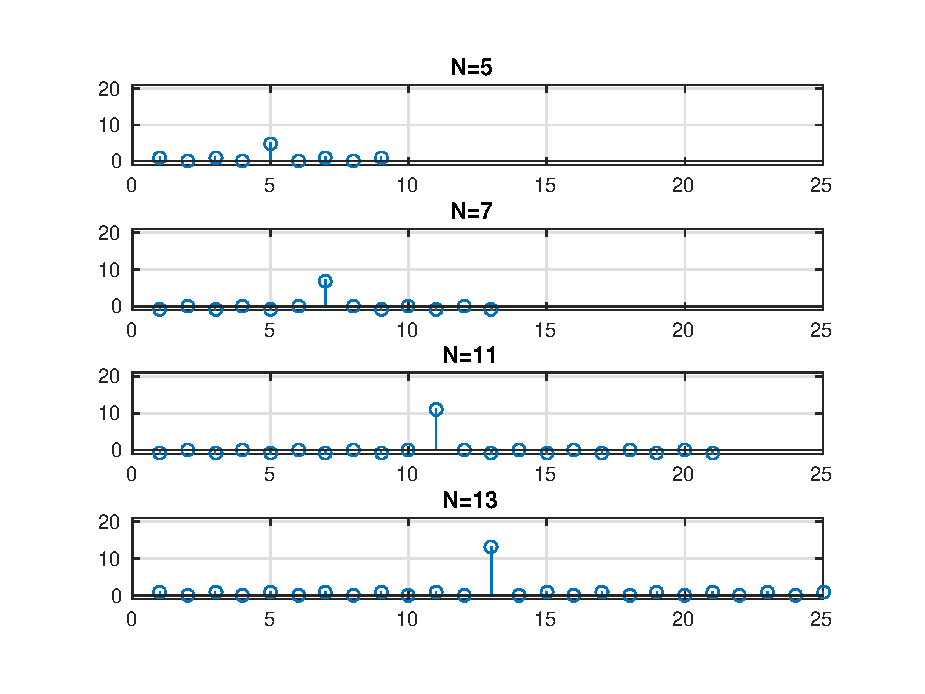
\includegraphics[width=0.8\textwidth]{barkerCodes.eps}
\caption{Barker code autocorrelations for different lengths.}
\end{figure}
%
\begin{table}[ht!]
\centering
\caption{Barker Codes From \texttt{comm.BarkerCode}}
\label{tbl:barkercode}\vspace*{3mm}
\begin{tabular}{l|l}
 N & \multicolumn{1}{c}{Code} \\ \hline
 2 & $-1,\, +1$ \\
 3 & $-1,\, -1,\, +1$ \\
 4 & $-1,\, -1,\, +1,\, -1$ \\
 5 & $-1,\, -1,\, -1,\, +1,\, -1$ \\
 7 & $-1,\, -1,\, -1,\, +1,\, +1,\, -1,\, +1$ \\
 11 & $-1,\, -1,\, -1,\, +1,\, +1,\, +1,\, -1,\, +1,\, +1,\, -1,\, +1$ \\
 13 & $-1,\, -1,\, -1,\, -1,\, -1,\, +1,\, +1,\, -1,\, -1,\, +1,\, -1,\, +1,\, -1$ \\
\end{tabular}
\end{table}

\newpage
\section{Open-ended Design Problem: Full Frame Recovery}

%NEW SYSTEM DIAGRAM WITH SYNCHRONIZERS
%
%COMBINE COARSE AND FINE FREQUENCY CORRECTION IS APPROPRIATE FASHION AND DESCRIBE REASONING


\subsection{Objective}
The objective of this problem is to design and implement a
software-defined radio (SDR) communication system capable of
automatically transmitting and recovering full frames between two Pluto
SDRs.

In Sections~\ref{sec:timing} you have implemented and simulated frame estimation.  
Now we will introduce the Pluto to deal with realistic sample offset behavior.  To simplify this process a set of required tasks are staged to gradually increase the difficulty of the overall implementation.  We have presented a method for sample offset estimation, but you are free to use these in any arrangement you want, or use your own algorithms.  However, you must 
provide an evaluation of the overall system performance.  Your final implementation should be tuned to handle 
any set of Pluto radios, not just the ones used by your team.\par
%
With your implementation perform the following tasks:
%
\begin{enumerate}
 \item First, using a single Pluto transmit your DBPSK or QPSK reference signal across to the same radio.  Ignore timing correction and frequency correction for now, since they should be minimal.  Provide packet error rate results for this implementation.
\item Repeat this experiment but include your frequency correction implementation and manually introduce an offset at the transmitter.  Provide packet error rate results.  You should observe initial errors during the lock period of the PLL.
\item Next, reset your transmitter and receivers to have identical frequencies again.  Now insert your timing estimation design from lab 2, and provide packet error rate results here.
\item Finally, if you have had reasonable packet error rate result so far  using a pair of Plutos repeat this estimation again as previously performed with a single Pluto.  Provide packet error rates again.
\end{enumerate}
%

% \subsection{Theoretical Background}
% \begin{enumerate}
% \item Before you apply your method to USRP2 boards, it is highly recommended that you test your method with Simulink-only model without USRP and see whether it works.
% \item In the Simulink-only model, you can introduce the frequency offset by \texttt{Phase/Frequency Offset} block. Specify a frequency offset in this block, and see whether
% your Simulink model can give you the number you have specified.
% \item An important hint: If you take the square of a signal, the FFT of the received signal will be shifted double of the frequency offset.
% \item In your model, you might need the following blocks:
% \begin{enumerate}
% \item \texttt{Random Integer Generator}
% \item \texttt{Baseband Modulator}
% \item \texttt{Raised Cosine Transmit Filter}
% \item \texttt{Magnitude FFT}
% \item \texttt{Probe}
% \item \texttt{Maximum}
% \end{enumerate}
% The first three blocks are used on the transmitter side, and the
% last three blocks are used on the receiver side. Using
% \texttt{Probe} and \texttt{Maximum}, you will be able to find the
% location of the peak of the FFT. But of course, you are not
% constrained to these blocks. You can use all the blocks available in
% Simulink. If you want, you can even use MATLAB to implement your
% method.
% \item Although you are required to find the frequency offset of two USRP2 boards, you are actually trying to find the frequency offset of the received signal.
% \item Compare your result here from what you have obtained in Section~\ref{sec:offset}.
% \end{enumerate}
%
% \newpage

\section{Lab Report Preparation \& Submission Instructions}
Include all your answers, results, and source code in a laboratory
report formatted as follows:
\begin{itemize}
 \item Cover page: includes course number, laboratory title, names and student numbers of team, submission
 date.
 \item Table of contents, list of tables, list of figures.
 \item Commentary on designed implementations, responses to laboratory questions, and explanation of
 observations.
 \item Responses to open-ended design problem.
 \item Source code (as an appendix).
\end{itemize}

Remember to write your laboratory report in a narrative approach, explaining your experience and observations in such a way that it provides the reader with some insight as to what you have accomplished.  Furthermore, please include images and outputs wherever possible in your laboratory report document.\\

\noindent Each group is required to submit a single report
electronically (in PDF format) to \texttt{alexw@ece.wpi.edu} by the scheduled due date and time.
Reports that do not meet these specifications will be returned
without evaluation and will receive a grade of ``0'' for the report
segment of the laboratory experiment.


\newpage
\bibliographystyle{plain}
\bibliography{lab1bib}


\end{document}
